\documentclass[a4paper,12pt]{article}
\usepackage{amsmath,amsfonts,amsthm,amscd,amssymb,latexsym,eufrak}
%%%%%%%%%%%%%
\usepackage{enumerate,graphicx,psfrag,subfigure}%,jchangebar,oldgerm}
\usepackage[mathscr]{eucal}
\usepackage[usenames]{color}
\usepackage{url}
\usepackage{comment}
%\usepackage{showkeys}
%%%%%%%%%
\sloppy

%%\documentclass[12]{article}


%%%%%%%%%%%%%%%%%%%%%%%
%
%
%
\title{The subgroup membership problem
}
\author{Andrew J. Duncan, Elizaveta Frenkel}

%%%%%%%%%%%Liza to compile
%\newtheorem{theorem}{Theorem}[section]
%\newtheorem{maintheorem}{Theorem}[]
%\newtheorem{lemma}[theorem]{Lemma}
%\theoremstyle{definition}
%\newtheorem{algorithm}[theorem]{Algorithm}
%\newtheorem{corollary}[theorem]{Corollary}
%\newtheorem{conjecture}[theorem]{Conjecture}
%\newtheorem{definition}[theorem]{Definition}
%\newtheorem{example}[theorem]{Example}
%\newtheorem{problem}[theorem]{Problem}
%\newtheorem{question}[theorem]{Question}
%\newtheorem{remark}[theorem]{Remark}
%\newtheorem{proposition}[theorem]{Proposition}
%\newtheorem{convention}[theorem]{Convention}
%\newtheorem{comment[theorem]{Comment}
%\newtheorem{claim}[theorem]{Claim}
%%\newtheorem{procedure}{Procedure}%[theorem]%[section]
%\newtheorem{procedure}{Procedure}[section]%[theorem]
%%%\newtheorem{proof}[proof]{Proof}
%%%%%%%%%%%Liza to compile



%%%%%%%%%%%%%%%%%%%%%%%%%%%
%%%%%%%%%%%%%%%%%%%%%%%%%%%
\renewcommand{\a}{\alpha }
\renewcommand{\b}{\beta }
\newcommand{\G}{\Gamma }
\newcommand{\g}{\gamma }
\newcommand{\D}{\Delta }
\renewcommand{\d}{\delta }
%\def\vd{\vardelta}
\newcommand{\ep}{\epsilon }
\newcommand{\e}{\varepsilon }
\newcommand{\z}{\zeta }
%\eta
\renewcommand{\th}{\theta }
\newcommand{\T}{\Theta }
\renewcommand{\i}{\iota }
\renewcommand{\k}{\kappa }
\renewcommand{\l}{\lambda }
\renewcommand{\L}{\Lambda }
%\mu
%\nu
%\xi
%omicron
%\pi
\renewcommand{\r}{\rho }
\newcommand{\s}{\sigma }
\renewcommand{\S}{\Sigma }
\renewcommand{\t}{\tau }
\newcommand{\up}{\upsilon }
\newcommand{\U}{\Upsilon }
%\phi
\newcommand{\x}{\chi }
%\psi
\newcommand{\W}{\Omega }
\newcommand{\w}{\omega }
%%%%%%%%%%%%%%%%%%%%%%%%%%%%%%%
%%%%%%%%%%%%%%%%%%%%%%%%%%%%%
\newcommand{\pd}{\partial}
\newcommand{\wht}{\widehat}
%\newcommand{\cC}{{\mathcal C}}
%\newcommand{\cdim}{\texttt{cdim}}
\newcommand{\fC}{{\textswab C}}
\newenvironment{ef}{\noindent\color{blue} \bf EF: }{}
%
\newcommand{\cA}{{\cal{A}}}
\newcommand{\cD}{{\cal{D}}}
\newcommand{\cF}{{\cal{F}}}
\newcommand{\cH}{{\cal{H}}}
\newcommand{\cJ}{{\cal{J}}}

\newcommand{\cK}{{\cal{K}}}
\newcommand{\cP}{{\cal{P}}}
\newcommand{\cR}{{\cal{R}}}
\newcommand{\cS}{{\cal{S}}}
\newcommand{\cW}{{\cal{W}}}
\newcommand{\cQ}{{\cal{Q}}}
%\newcommand{\GG}{\ensuremath{\mathbb{G}}}
\newcommand{\pp}{\mathbf{p}}
%%%%%%%%%%%%%%%%%%%%%%%%%%%%%%
\newcommand{\nul}{\emptyset }

%%%%%%%%%%%%%%%%%%%%%%%%%%%%%%
\newtheorem{theorem}{Theorem}[section]
\newtheorem{lemma}[theorem]{Lemma}
\newtheorem{corollary}[theorem]{Corollary}
\newtheorem{proposition}[theorem]{Proposition}
\newtheorem{axiom}[theorem]{Axiom}
\newtheorem{definition}[theorem]{Definition}
\newtheorem*{defn*}{Definition}
\newtheorem{conjecture}[theorem]{Conjecture}
%cvs -d :pserver:najd2@cvs.mas.ncl.ac.uk:/CVS/najd2
\newtheorem{exam}[theorem]{Example}
%\newtheorem{comment}[theorem]{Comment}
%
%
\newenvironment{example}{\begin{exam} \rm}{\end{exam}}
%
%
%
\newtheorem{remk}[theorem]{Remark}
\newenvironment{remark}{\begin{remk} \rm}{\end{remk}}
%
%%%%%%%%%%%%
\numberwithin{equation}{section}
\numberwithin{figure}{section}
%%%%%%%%%%%%%%%%%%%%
\newcommand{\Iso}{\operatorname{Isom}}
\newcommand{\Aut}{\operatorname{Aut}}
%%%%%%%%%%%%%%%%%%%
\renewcommand{\AA}{\ensuremath{\mathbb{A}}}
\newcommand{\ZZ}{\ensuremath{\mathbb{Z}}}
\newcommand{\QQ}{\ensuremath{\mathbb{Q}}}
\newcommand{\RR}{\ensuremath{\mathbb{R}}}
\newcommand{\NN}{\ensuremath{\mathbb{N}}}
\newcommand{\CC}{\ensuremath{\mathbb{C}}}
\newcommand{\FF}{\ensuremath{\mathbb{F}}}
%\renewcommand{\ker}{\verb"Ker"}
\newcommand{\cC}{\mathcal{C}}
\renewcommand{\cF}{\mathcal{F}}
\newcommand{\cO}{\mathcal{O}}
\renewcommand{\cS}{\mathcal{S}}
\newcommand{\la}{\langle}
\newcommand{\ra}{\rangle}
%\newcommand{\BA}{\ensuremath{\mathbb{A}}}
%%%%%%%%%%%%%%%%%%%%%%%%%%%%%%%%%%%%%%
\newcommand{\maps}{\rightarrow}
\newcommand{\ov}[1]{\overline{#1}}
\newcommand{\bs}{\backslash}
%%%%%%%%%%%%%%%%%%%%%%%%%%%%%%%
\newcommand{\be}{\begin{enumerate}}
\newcommand{\ee}{\end{enumerate}}
\newcommand{\bd}{\begin{description}}
\newcommand{\ed}{\end{description}}
%%%%%%%%%%%%%%%%%%%%%%%%%%%%%%%%%%%
%
\newenvironment{ajd}{\noindent\color{blue} AJD }{}
\newenvironment{xxx}{\noindent\color{red}}{}
%
\begin{document}
\maketitle

\begin{abstract}
We modify Stallings folding theory to apply it to amalgamated
products of finite rank free groups. Using special kind of normal
forms, we show how they can be used to decide subgroup membership
problem for free products with amalgamation.
 \end{abstract}



\section{Introduction}\label{se:global_intro}
%%Lisa's test
Stallings introduced his technique of foldings in his paper
\cite{stallings83} where he applied this technique to investigate
free groups. In his \cite{stallings88} Stallings extend ideas of
foldings to non-free actions of groups on graphs and trees. Next
years ideas of Stallings was widely generalized in different
directions and applied to decide different problems in
combinatorial group theory, see for example
\cite{befe,BoWei,KM02,SilvaWeil08}.

Let $G = <X|R>$ be a finitely generated group. The group $G$ has
solvable membership problem if there is an algorithm which, for
any finite set of words $w, k_1, \ldots k_s$ in $G$ decides
whether or not the element $w$ belongs to the subgroup $K = <k_1,
\ldots, k_s>$. In this paper we decide the subgroup membership
problem for amalgamated products of finite rank free groups, using
a language of special normal forms for elements of such groups and
extending ideas of Stallings foldings for this group construction.
Free group constructions, in particular, free products of groups,
with or without amalgamation, $HNN-$extensions
 and, more generally, fundamental groups
of graphs of groups represent a subject of special interest in
group theory from different points of view. First results here
related to the solvability of membership problem in group
constructions described above is due to Mihailova (see
\cite{mi59,mi68}), who shown that the membership problem is
decidable in free product of groups $A$ and $B$ if it is decidable
in both factors. One should mention also another famous result of
Mihailova \cite{mi58} which provide an important counter-example
in this direction. Namely, she constructed a finitely generated
subgroup of direct product of two free groups of rank two with
unsolvable membership problem; notice also, that this direct
product can be considered also as sequence of two $HNN-$extensions
of rank two free group. On the other hand, it is another classical
result that a free group of finite rank has solvable (uniform)
membership problem. It shows, that even innocent group
constructions can affect solvability of the membership problem
dramatically.

The membership problem for free products with amalgamation and
$HNN-$extension was studied by Bezverkhnii in his papers
\cite{bez81,bez86,bez90,bez91}, where he used combinatorial
technique and standard normal forms in amalgamated product of
groups. Our approach is, first of all, more geometrical, and since
we have an eye on generalization of this result on other free
constructions, we were obliged to introduce another language to
study these constructions. Another significant step in this
direction was done by Kapovich, Miasnikov and Weidmann in their
paper \cite{KMW03}, where authors investigated uniform membership
problem for fundamental groups of graph of groups under certain
assumptions on both vertices and edges groups. In particular, they
shown that for the case where all vertices groups either locally
quasiconvex wordhyperbolic or polycyclic-by-finite and all edges
groups are polycyclic-by-finite the uniform membership problem for
fundamental groups of such a graph of groups is solvable.

As it was mentioned above, we want to introduce geometric
technique, which relies on Stallings foldings ideas and another
type of normal forms for elements of amalgamated products of
groups. Now, a few words on the structure of the paper. In Section
\ref{sec:intro} we introduce the double coset normal forms for
elements amalgamated products of finite rank free groups.
 In Section \ref{sec:dcforms} we study the structure of these double coset normal forms and describe the explicit procedure
 of their construction. Namely, we show how to obtain a unique normal form of an element in a free group of finite
 rank; these forms are based on double coset of representatives of
 two types representatives (see subsection \ref{sub:2cosetrepr}).
 Simple procedure described in the beginning of \ref{sec:foldings}
 shows how to rewrite arbitrary word in a reduced form into double
 coset normal form using these special representations in factors.

Section  \ref{sec:foldings} is the heart of the paper. Let $K$ be
a subgroup of an amalgamated product of finite rank free groups.
Using the notion of double coset graph (automaton), we extend
folding procedure such the after the sequence of transformations
of double coset graph for $K$ the resulting graph recognize
precisely normal forms of elements of $K$.



Authors are grateful to Vladimir Remeslennikov for helpful
discussions and to Christian Perfect who did something.{\ef Should
we mention VNR here or among the authors? What should we say about
Christian's work?}



\section{Double coset normal form}\label{sec:intro}
Based on notes copied (laboriously) from Christian's page
\url{
http://checkmyworking.com/misc/writemaths/?doublecoset
}

$F_1$, $F_2$ free groups (finitely generated by $X_1$
and $X_2$, respectively).

Let $H_1 \leq F_1$, $H_2 \leq F_2$ such that
there exists an isomorphism $\phi: H_1 \rightarrow H_2$.

i.e. we have finite bases $\{h_1, \ldots, h_m \}$  for $H_1$ and
$\{h_1', \ldots, h_m'\}$ for $H_2$.

Consider the free group $F(Z)$, generated by $Z=\{z_1, \ldots, z_m\}$,
and the maps $\phi_1$ and $\phi_2$ such that
$\phi_1(z_i)=h_i(X_1)  $ and  $\phi_2(z_i)=h^\prime_i(X_2)$, $i=1,\ldots ,m$.
Thus $\phi_i$ extends to an isomorphism of $F(Z)$ to $H_i$. We choose
the $\phi_i$ so that $\phi=\phi_2\phi_1^{-1}$.

Let ${G = F_1 \underset{H_1=H_2}{\ast} F_2}$, the group with
 presentation \[\la X_1,X_2 | h_i = h_i', i=1, \ldots ,m\ra.\]

A  set $S_i \subseteq F_i$ such that
\be
\item
$F_i = \displaystyle{\bigcup_{s \in S_i} H_isH_i}$
and
\item
for all $s, s^\prime \in S_i$, $s\in H_i s^\prime H_i$
implies $s=s^\prime$,
\ee
is called a set of \emph{double coset representatives for} $H_i\le F_i$.

Let $S_1$ and $S_2$ be sets of  double coset representatives of
$H_1\le F_1$ and $H_2\le F_2$, respectively. Let $g \in G$.
A word $w$ representing $g$ is in \emph{(double coset) normal form} if
$w = h_{0}p_1h_{1}p_2 \cdots h_{k-1}p_kh_{{k}}$, $k\ge 0$,  with
\be
\item $p_i \in S_1\cup S_2$  and $h_i$ is a reduced word in $F(Z)$ and
\item if $p_i\in S_j$ then $p_{i+1}\notin S_j$, for $j=1$ and $2$,
\ee
for $i = 1, \ldots ,k$.


\section{Constructing double coset representatives}\label{sec:dcforms}

Given an arbitrary word $g\in F_1\ast F_2$,
we should like an algorithm to write $g$ in double coset normal form
with respect to some choice of double coset representatives. We may
assume (after free cancellation if necessary) that $g$ is a
reduced word in $((X_1\cup X_2)\cup ( X_1^{-1}\cup X_2^{-1}))^\ast$.

First we say $g$ is in \emph{reduced form} if $g = g_1 \cdots g_t$, where
$g_1 \in F_1$ or $g_1 \in F_2$ and
for
$i > 1$,    $g_i \in (F_1 \backslash H_1)\cup (F_2\backslash H_2)$ and  $g_i$
and  ${g_{i+1}}$ belong to  different factors. As $F_1$ and
$F_2$ have solvable subgroup membership problem we can write $g$ in
reduced form. More precisely, we construct a Stallings automaton
(see below) $A_k$ for
$H_k\le F_k$. % and choose a maximal subtree $T_k$ of $A_k$, $k=1,2$.
Then we write $g=f_1\cdots f_r$, in free product normal
form (each $f_i$ is in a factor and successive terms are
from different factors).
Now,
using the appropriate Stallings automaton $A_k$, we write $f_r=h_rg_r$, where
$h_r$ is the maximal prefix of $f_r$ accepted by $A_k$ and $g_r$ is
 the
unique word such that $f_r=h_rg_r$, reduced as written.

Using the maps $\phi_1$ and $\phi_2$ we now write $h_r$ in terms of the
generators of the other factor, to obtain $h^\prime_r$ and then
replace $f_{r-1}$ with $f_{r-1}^\prime=f_{r-1}h^\prime_r$. Now start again with
$f_{r-1}^\prime$ instead of $f_r$. Continue till the word is exhausted.
This gives $g=g_1\cdots g_t$ in reduced form.

To rewrite in double coset normal form we need to
 rewrite
each $g_i$ in double coset normal form in its factor, with respect
to some (fixed) set of double coset representatives. We show how
this can be done below.

\subsection{Automata and Stallings Foldings}\label{sub:foldings}
%{\bf We should include a short description of Stallings folding, as in
%Enric's notes from Manresa \cite{ventura11}.} \\[1em]

An {\em automaton} $A$ is  a quintuple
$(\S,Q,\d,\mathcal{S},\mathcal{F})$, where $\S$ is finite set
called the {\em alphabet}, $Q$ is a finite set of {\em states},
$\d$ is a map $\d:Q\times \S\maps Q$, called the {\em transition
function}, $\mathcal{S}\subset Q$ is the (non-empty) set of {\em
start states} and $\mathcal{F}\subseteq Q$ is the set of {\em
final states}. (Usually $\mathcal{S}$ is a singleton.) If
$\mathcal{F}=\{s_0\}=\mathcal{S}$ it's common to drop
$\mathcal{F}$ from the description and define $A$ as a quadruple.

 
By a graph we mean a finite, directed, edge labelled graph. 
We shall associate to an automaton $A$
a graph $\G_A$ with vertices
$V=V(\G_A)=Q$; edge set $E=E(\G_A)$ consisting of elements
$(u,\s,v)$ of $Q\times \S\times Q$ such that $\d(u,\s)=v$; and
labelling function $l:E\maps \S$ given by $l(u,\s,v)=\s$, for all
$(u,\s,v) \in E$.  If $\mathcal{S}$ and $\mathcal{F}$ are the sets
of start and final states of $A$ we sometimes write
$(\G_A,\mathcal{S},\mathcal{F})$ for
$(\S,Q,\d,\mathcal{S},\mathcal{F})$, and in addition if
$\mathcal{S}=\{s_0\}$ and $\mathcal{F}=\{f_0\}$, we may abbreviate 
this to $(\G_A,s_0,f_0)$. If $\mathcal{S}=\{s_0\}=\mathcal{F}$ 
we 
call $s_0$ the {\em root}
vertex of $\G_A$ and say that $A$ and $\G_A$ are {\em rooted}. We may
 write $(\G_A,s_0)$ for $(\G_A,s_0,f_0)$ if this is the case.  For notational simplicity we identify $\G_A$
and $A$ whenever it is convenient and unambiguous. 


The
label $l(p)$ of a path is the concatenation of the labels of the
edge sequence of $p$.  If $w$ is the label of a path 
in $\G_A$, from a vertex of $\cS$ to a vertex of $\cF$, then we
say that $w$ is accepted by $A=(\G_A,\cS,\cF)$. The set of all
words in the free monoid $\S^*$, generated by $\S$, which are 
accepted by $A$  is called
the {\em language accepted by} $A$ and denoted $L(A)$. 
We extend this terminology, for an automaton 
$A=(\S,Q,\d,\mathcal{S},\mathcal{F})$,  
to say that a  word $w$ is {\em readable} 
by $A$ if $w$ is in the
language accepted by $(\G_A,\cS,Q)$.  
If $\S$ is a
subset of a group $G$
 then the  natural map from $L(A)$ to
$G$ is denoted $\pi:L(A)\maps G$.



An {\em involutive alphabet} is a set $\S$ of the form $\{a_1, \ldots, ,
a_r, a_1^{-1}, \ldots, a_r^{-1}\}$.
The automaton $A =(\S, Q, \d,\mathcal{S},\mathcal{F})
= (\G_A, \mathcal{S}, \mathcal{F})$ is {\em
involutive} if $\S$ is an
involutive alphabet and, for all $p, q \in Q$ and $a \in \S$,
$\d(p,a)=q$ if and only if $\d(q, a^{-1})=p$ (that is $(u, \s, v) \in E
\Leftrightarrow (v, (\s)^{-1}, u) \in E$). From now we will
consider involutive automaton only. The automaton $A$ 
is {\em deterministic}  or {\em folded} if $\d(p,a)=q$ and
$\d(p,a)=q'$ imply $q=q'$ (that is, $(u, \s, v)
\in E$ and $(u, \s, v^\prime) \in E$ imply $v=v^\prime$). A rooted
automaton $A= (\G_A, s_0)$ is called {\em trim} if it has no
vertices of degree $1$ except maybe $s_0$. Finally, an involutive, rooted, 
deterministic, trim automaton, with a single final state, is called 
an {\em inverse} automaton. 

Since we identify the automaton $A$ with the graph $\G_A$, we ascribe
properties of automata (like rooted, trim, involutive, folded or
inverse) to graphs in general and $\G_A$ in particular.

%%Let $A=(V,E,s_0)$ and $A^\prime=(V^\prime,E^\prime,s^\prime_0)$ be
%%two automata. A {\em morphism} $A \rightarrow A^\prime$ is a map
%%$\varphi: V \rightarrow V^\prime$ such that $\varphi(s_0) =
%%s^\prime_0$ and $(p,a,q) \in E \Rightarrow
%%(\varphi(p),a,\varphi(q)) \in E^\prime$.
We now recall the notion of a Stallings folding of an
automaton, which we will use directly, to construct Stallings 
automata for subgroups of free groups, and in generalized form
to produce dc-resolutions of automata (in Section
\ref{sec:foldings}). For more details of Stallings foldings  and  Stallings 
automata  see \cite{ventura11} or \cite{BartholdiSilva}.

An {\em elementary folding} of a rooted, directed, labelled 
graph $(\G,s_0)$ is a
graph $(\G^\prime,s^\prime_0)$ obtained from $(\G,s_0)$ as
follows. Suppose that $e=(u, \s, v)$ and $e^\prime=(u, \s,
v^\prime)$ are edges of $\G$. (We do not require $u$, $v$ and
$v^\prime$ to be distinct.)
 Then $\G^\prime$ is the quotient of $\G$ formed by identifying
$v$ and $v^\prime$, to form a new vertex $v^{\prime\prime}$; and
$e$ and $e^\prime$, to form a new edge $e^{\prime\prime}=(u, \s,
v^{\prime\prime})$. If $s_0= v$ or $s_0 = v^\prime$ then
$v^{\prime\prime}$ is the root of $\G^\prime$ and otherwise
$s^\prime_0=s_0$.
 A {\em folding} of a graph $\G$ is a graph obtained
from $\G$ by a finite sequence of elementary foldings. 

If a rooted graph $\G$ is not folded then a folding may be applied; reducing the 
number of edges of the graph. Continuing this way a folded graph may eventually 
be produced. It follows that  folded graphs are precisely those 
to which no elementary folding may be applied. 

A morphism of  rooted 
graphs $\G$ and $\G^\prime$ is a map $\theta: \G\maps \G^\prime$ 
which maps vertices to vertices and edges to edges in such a way
that
\be
\item if $s$ is the root of $\G$ then $\theta(s)$ is the root of 
$\G^\prime$ and 
\item  if $(u,\sigma,v)$ is an edge of $\G$ then 
$\theta(u,\sigma,v)=(\theta(u),\sigma,\theta(v))$. 
\ee
An elementary
folding of  $(\G,s_0,t)$ to  $(\G^\prime,s^\prime_0, t^\prime)$ induces a morphism
from $\G$ to $\G^\prime$: namely the quotient map. Therefore there is
 a uniquely determined {\em folding morphism} from $\G$ to any folding. Moreover, if $\G_1$
is a folding of $\G$ and $\theta$ is the folding morphism then $\pi(L(\G,s,t))=
\pi(L(G_1,\theta(s),\theta(t)))$.   


Let $X$ be a finite alphabet, $F=\FF(X)$ and $H$ a finitely generated subgroup
of $F$.  By a {\em reduced} word we mean
 a freely reduced word in $(X\cup X^{-1})^\ast$, and we write $w\in \FF(X)$
to mean that $w$ is a reduced word. For $u,v, w\in F(X)$ we
write $w=u\circ v$ if $|w|=|u|+|v|$, in which case we say that $u$ is a {\em prefix}
of $w$. 

Let $Y=\{w_1,\ldots ,w_n\}$ be a generating set for $H$, where $w_i\in F$. 
The {\em flower automaton} $\G_Y(H)$, of $H$ (with respect to this generating set)
is the graph constructed as follows. For each $i$ let $C_i$ be a cycle
graph with $|w_i|$ vertices, and choose a vertex $v_i$ as the root. Direct
and label the edges of $C_i$, with elements of $X$,  
so that the simple closed path based at $v_i$ has
label $w_i$ (read in, say, a counter-clockwise direction). The flower
automaton $G_Y(H)$ is formed by identifying all the vertices $v_i$ to form 
a new graph, with root $v$ the image of the $v_i$. If $L_Y$ is the language  accepted
by $(\G_Y(H), v)$ then $\pi(L_Y)=H$. 
 

The flower automaton of $H$ depends on the chosen generating set, and is, 
in general,
non-deterministic (at the root vertex). Stallings \cite{stallings83} 
proved that the folded graph $\G(H)$, obtained by applying foldings to the 
flower automaton of $H$, is  independent of the generating set chosen, and
is inversive.
As folding does not affect the image of the map $\pi$, it follows that, if
$s$ is the root of $\G(H)$ and $L$ is the language accepted by $(\G(H),s)$ 
then 
$\pi(L) =H$. 
Moreover  
every reduced word representing an element of $H$ belongs to $L$.
\begin{definition}
The automaton $(\G(H),s)$ is  called the {\em Stallings automaton} of $H$. 
\end{definition}
\subsection{Double coset representatives}\label{sub:2cosetrepr}
Let $X$ be a finite alphabet, $F=\FF(X)$ and $H$ a finitely generated subgroup
of $F$. 

Let $A$ be the Stallings automaton for $H$, and let  $s_0 =
1$ be its start state. 
As $A$ is inversive, if $w$ is readable by $A$ then there exists a
unique vertex  $\t(w)$ of $\G_A$ such that $w$ is accepted by 
$(\G_A,s_0,\t(w))$: we call $\t(w)$ the {\em terminal vertex} of $w$. ($L$ is the set of words $w$ readable by $A$ with 
$\t(w)=1$.) 

Fix a spanning tree $T$ for $A$. For each vertex $v$ of $A$
let $w(v)$ denote the label of the path from $s_0=1$ to $v$ in
$T$.  Define
\[L_T=\{w(v): v \textrm{ is a vertex of } A\}\]
and 
\[L_Q=\{w:w \textrm{ is readable by } A\}.\]
If $w, s, u\in F(X)$ with $w=s\circ u$ then we say that $s$ is 
\be[(i)]
\item
 an $L_Q${\em -prefix} of $w$ if $s\in L_Q$;  
\item 
an % {\em maximal}
$L_T${\em -prefix} of $w$ if $s\in L_T$.
\ee
An $L_Q$ or $L_T$-prefix $s$ of $w$ is  {\em maximal} if no longer
subword of $w$ is an $L_Q$ or $L_T$-prefix, respectively. 

We shall define a set of double coset representatives for $H$ in two parts.
We begin with the definition of the first type of representative. 
\begin{definition}[Double coset representative, type 1]
A a word $w\in F(X)$ is a {\em (double coset) representative of type} $1$ if
\[w=s\circ e \circ t^{-1},\]
where $e\neq 1$, $s$ is a maximal $L_Q$-prefix and an $L_T$-prefix of $w$, 
and $t$ is a maximal $L_Q$-prefix and an 
$L_T$-prefix of $t\circ e^{-1}$. Let $S^{(1)}$ denote the set of all representatives of type $1$.
\end{definition}

{\ef Notions of $L_T$-prefixes, maximal prefixes etc are closely related to the theory of (usual) coset
 representatives and there are a lot of things known about them (one-to-one correspondence between them and spanning subtrees etc. etc).
 We don't need to replace this definition since it looks convenient and compact, but, probably, we should refer reader to it... what do you think?
}



To describe the remaining representatives we shall first define an equivalence
relation on the ordered pairs of distinct vertices of $A$. Let
\[P=\{(u,v)\in V(A)\times V(A): u\neq v\}.\]
Define a relation $\sim$ on $P$ by $(u_0,u_1)\sim (v_0,v_1)$ if and only if
there exist paths $p_0$ and $p_1$ in $A$, from $u_0$ to $v_0$ and $u_1$ to $v_1$
respectively, such that $l(p_0)=l(p_1)$. (We allow these paths to have length $0$.)
It is easy to verify that $\sim$ is an equivalence relation on $P$.

\begin{lemma}\label{lem:equiv_verts}
Let $(u_0,u_1)$ and $(v_0,v_1)$ be elements of $P$ and let
$a_0=w(u_0)$, $a_1=w(u_1)$, $b_0=w(v_0)$ and $b_1=w(v_1)$. Then
$(u_0,u_1)\sim (v_0,v_1)$ if and only if there exist $h_0,h_1\in H$ such that
\[a_0a_1^{-1}=h_0b_0b_1^{-1}h_1^{-1}.\]
\end{lemma}
\begin{proof}
$\Rightarrow$: Let $p_0$ and $p_1$ be paths, from $u_0$ to $v_0$ and $u_1$ to $v_1$
respectively, such that $l(p_0)=l(p_1)=c$, say. Set $h_0=a_0cb_0^{-1}$ and
$h_1=a_1cb_1^{-1}$. Since $h_0$ and $h_1$ are labels of closed paths in $A$, based at $1$, we
have $h_0$ and $h_1$ in $H$. Thus
$a_0a_1^{-1}=h_0b_0c^{-1}cb_1^{-1}h_1^{-1}=h_0b_0b_1^{-1}h_1^{-1}$, as required.

$\Leftarrow$: Let $h_0$, $h_1 \in H$ such that $a_0a_1^{-1}=h_0b_0b_1^{-1}h_1^{-1}$.
Set $k=a_0^{-1}h_0b_0=a_1^{-1}h_1b_1$. Then $h_0=a_0kb_0^{-1}$ and $h_1=a_1kb_1^{-1}$
belong to $H$ so there exist paths $p_0$ and $p_1$ in $A$,
from $\t(a_0)=u_0$ to $\t(b_0)=v_0$ and
$\t(a_1)=u_1$ to $\t(b_1)=v_1$, both with labels $k$.
Therefore $(u_0,u_1)\sim (v_0,v_1)$.
\end{proof}

%%{\ef
%%It seems like we should specify different cases , depending on
%%$u_0, v_0$ and $u_1,v_1$ belonging to the same loop $h_i$ or not;
%%or something like this. Take an equivalence class as in example
%%\ref{ex:f_1f_2}. Then $a_0 = y_2^{-1}y_1$, $a_1 = y_1^2$, $b_0 =
%%y_2^{-1}$, $b_1=y_1$. Further, we obtain $c = y_1$ and the
%%equality satisfies, but with elements $h_0 = y_2^{-1} y_1^2 y_2$
%%and $h_1 = y_1^2$ which are not in $H_2$, as far as I understand.
%%Am I right or I misunderstood something?
%%}

To work with the equivalence relation $\sim$ its useful to define
the product of graphs. Given (labelled, directed) 
graphs $\G_1$ and $\G_2$ we define the {\em
product} graph $\G_1\times \G_2$ to be the graph with vertices
$V=V(\G_1)\times V(\G_2)$ and with a directed edge labelled $a$
from $(u_1,u_2)$ to $(v_1,v_2)$ if and only if there are edges
$(u_1,a, v_1)$ and $(u_2,a,v_2)$ in $\G_1$ and $\G_2$,
respectively. If $\G$ is a graph then 
vertices of $\G\times \G$ of 
 the form $(v,v)$ are called {\em diagonal vertices}. 
% We call the graph formed from  $\G\times \G$ by removing  
% the diagonal vertices (and all incident edges) the 
%{\em non-diagonal subgraph of} $\G\times \G$. 
Note that if
$\G$ is folded there is no edge of $\G\times \G$ 
joining a diagonal vertex to a non-diagonal
vertex. In this case it 
follows that the diagonal vertices are the vertices of a 
connected component of $\G\times \G$, which is isomporphic to $\G$, and 
that no other connected component contains a diagonal vertex. 

In this notation $P$ is the set of non-diagonal vertices of  
 of $\G_A\times \G_A$ and   
$(u,v)\sim (u',v')$ if and only if there is 
a path from $(u,v)$ to $(u',v')$ in $\G_A\times \G_A$.
 Thus, as $\G_A$ is folded,  the equivalence class of $(u,v)\in P$
is the set of vertices of the connected component of $\G_A\times \G_A$ 
containing $(u,v)$. 

We shall choose one double coset representative corresponding to
each $\sim$ equivalence class. First observe that if
$(u,v)\in P$ and $w(u)=a\circ x$, $w(v)=b\circ x$, for some
$a,b\in F(X)$ and $x\in X^{\pm 1}$, then $(\t(a),\t(b))\in P$ and
$(u,v)\sim (\t(a),\t(b))$. It follows that every equivalence  class
of $\sim$ contains an element $(u',v')$ such that
$w(u')w(v')^{-1}$ is a reduced word; and representatives of each
equivalence class will be chosen to have this property. 
%We make a choice $(u,v)$ of representative of each equivalence class
%of $\sim$ so that 
%$w(u)w(v)^{-1}=w(u)\circ w(v)^{-1}$), in the next definition.

\begin{definition}
Let $\pp$ be an equivalence
class of $\sim$ and let $Y$ be the set of all pairs $(u,v)\in \pp$
such that $|w(v)|$ is minimal (amongst elements of $\pp$). Choose
$(u,v)\in Y$ such that $|w(u)|$ is minimal (amongst elements of
$Y$) and define $(u,v)$ to be the $\sim$ {\em representative} of
$\pp$. %Fix one $\sim$ representative for each equivalence class of$\sim$ and 
Let $P_0$ denote the set of  all these $\sim$ 
representatives.

A word $w\in F(X)$ is
 a {\em (double coset) representative of type} $2$ 
if $w=w(u)w(v)^{-1}$, for some $(u,v)\in P_0$.
Let $S^{(2)}$ denote the set of all representatives of type $2$.

For each $(u,v)$ in $P$ choose a path in $\G_A\times \G_A$ 
from $(u,v)$ to the $\sim$ representative
$(u_0,v_0)$ of $(u,v)$ and define the {\em connecting element}
$c(u,v)$  of $(u,v)$ to be the label of this path.  
\end{definition}
The  connecting elements enable systematic rewriting of certain
elements of $\FF$ in terms of representatives of type 2, as will be
seen below.
\begin{definition}
Define $S=S^{(1)}\cup S^{(2)}$. 
\end{definition}


\begin{proposition}\label{prop:dcreps}
$S$ is a set of double coset representatives for $H$.
\end{proposition}
\begin{proof}
First we shall show that every element $w\in F(X)$ lies in $HdH$,
for some $d\in S$. In fact we describe an algorithm which
rewrites a given word $w$ in this form.

Assume that the Stallings automaton $A$ for $H$ has been constructed by folding from
given generators for $H$. A spanning tree $T$
for $A$ may then be chosen and the
set $L_T$ computed. 
To find the equivalence class of a pair $(u,v)\in P$ the 
graph $\G_A\times \G_A$ is constructed. By definition, $(u',v')\sim 
(u,v)$ if and only if there is a path in $\G_A\times \G_A$ from $(u',v')$
to $(u,v)$. Therefore the $\sim$ equivalence class of $(u,v)$ is the
vertex set of the connected component of $\G_A\times \G_A$ containing
$(u,v)$.   
Having constructed the equivalence classes of $\sim$
 a set of $\sim$ representatives may be constructed, by considering the
lengths of $w(a)$ and $w(b)$ for all $(a,b)$ in an equivalence class. Thus the
sets $P_0$ and $S^{(2)}$ may be computed.   \\

\noindent{\bf Algorithm I}:\\
Input $w\in F(X)$.
Let $h$ be the maximal prefix of $w$ accepted by $A$; so $h\in H$ and
$w=h\circ f$, for some $f\in F(X)$. Now use $A$ to find the maximal 
$L_Q$-prefix $p$
of $f$ (i.e. the maximal prefix readable by $A$). Then
  $f= p\circ q$, for some $q\in F(X)$.

Next find the maximal prefix $g$ of $q^{-1}$ acceptable by $A$: say
$q^{-1}=g\circ r$, for some $r\in F(X)$, and then the maximal $L_Q$-prefix
$t$ of $r$; say $r=t\circ e^{-1}$, for some $e\in F(X)$.

If $e\neq 1$ then
\[w=h\circ p \circ e\circ t^{-1}\circ g^{-1},\]
with $h,g\in H$. In this case $p$ and $t$ are readable by $A$. Set $y=w(\t(p))$
and $z=w(\t(t))$. Then $py^{-1}$ and $tz^{-1}$ belong to $H$. Moreover, as $p$
is the maximal $L_Q$-prefix of $f$ it is also the maximal
$L_Q$-prefix of $pet^{-1}$,  and so
  the
first letter of $e$ is not readable from the vertex $\t(p)=\t(y)$ of $A$.
In particular
$ye=y\circ e$. Similarly, the first letter of $e^{-1}$ is not readable from
the vertex $\t(t)=\t(z)$, so $ez^{-1}=e\circ z^{-1}$. Moreover $y$ is both 
a
maximal $L_Q$-prefix  and an $L_T$-prefix of $yez^{-1}$ and $z$ is a 
maximal $L_Q$-prefix  and an $L_T$-prefix of $ze^{-1}$.
Thus $yez^{-1}\in S^{(1)}$ and we output
\[w=(py^{-1}) (yez^{-1})(zt^{-1})\in HSH,\]
of the required form.

On the other hand if $e=1$ then
\[w=h\circ p\circ t^{-1}\circ g^{-1}.\]
In this case let $u=\t(p)$ and $v=\t(t)$,
let $(u_0,v_0)$ be the $\sim$ representative
of the equivalence class of $(u,v)$, $c=c(u,v)$, 
 $y=w(u_0)$ and $z=w(v_0)$. Then,  as in the proof of Lemma
\ref{lem:equiv_verts}, setting $h_0=w(u)cy^{-1}$ and
$h_1=w(v)cz^{-1}$ we have
 $h_0,h_1\in H$ and
\[w(u)w(v)^{-1}=h_0yz^{-1}h_1^{-1}.\] Furthermore
 $p w(u)^{-1}$ and  $t w(v)^{-1}$ are in $H$. Hence
\[
p\circ t^{-1}=( p w(u)^{-1})w(u)w(v)^{-1}( w(v)t^{-1})=( p w(u)^{-1}) h_0 yz^{-1}
h_1^{-1}( w(v)t^{-1})
\]
and by definition $yz^{-1}\in S^{(2)}$. We then output
\[w=a yz^{-1} b,\]
where $a=h ( p w(u)^{-1}) h_0=hpcy^{-1}\in H$ and $b=h_1^{-1}( w(v)t^{-1})g^{-1} 
=zc^{-1}t^{-1}g^{-1}\in H$.

It remains to show that if $s_0,s_1\in S$ with $s_1\in Hs_0H$
then $s_1=s_0$. Suppose that $s_1=as_0b$, where $a, b\in H$. If
$s_0\in S^{(1)}$, say $s_0=y_0e_0z_0^{-1}$, then, as $ay_0$ and
$b^{-1}z_0$ are readable by $A$ and $e_0\neq 1$, it follows (as
above) that $s_1$ cannot be factored as $s_1=yz^{-1}$, where both
$y$ and $z$ are readable by $A$. Hence both $s_0$ and $s_1$ belong
to $S^{(1)}$ or both belong to $S^{(2)}$.

Consider the case where both belong to $S^{(1)}$ and, in the usual notation,
$s_i=y_i e_i z_i^{-1}$, $i=0,1$. We have $s_1=as_0b$, $a,b\in H$, and as $y_0$ has
no left divisor in $H$, if $a\neq 1$ then $a$ does not cancel completely with
 a prefix of $y_0$. Thus, if $a\neq 1$ we may write $a=a_0\circ a_1$ and
$y_0=a_1^{-1}\circ y_0^\prime$, where $ay_0=a_0\circ y_0^\prime$. Since
$a$ is accepted by $A$ we have $\t(ay_0)=\t(a_0y_0^\prime)=\t(y_0)$. By definition
of $s_0$ the first letter of $e_0$ is not readable from the vertex $\t(y_0)$, so
it follows, as before that $a_0y_0^\prime e=a_0\circ y_0^\prime \circ e$. Similarly,
if $b\neq 1$ then $b=b_0\circ b_1$ and $z_0=b_0\circ z_0^\prime$, with
$z_0^{-1}b= (z_0^\prime)^{-1}\circ b_1$ and $e (z_0^\prime)^{-1}b_1=
e\circ  (z_0^\prime)^{-1}\circ b_1$. This implies that
$s_1=a_0\circ y_0^\prime \circ  e\circ  (z_0^\prime)^{-1}\circ b_1$ and by considering
maximal $L_Q$-prefixes of both sides we see that $y_1=a_0\circ y_0^\prime$ and
$z_1=b_1^{-1}\circ z_0^\prime$. We now have  $\t(y_1)=\t(a_0y_0^\prime)=\t(y_0)$ which
 means that
$y_0=y_1$ and this in turn implies that $a=1$. Similarly $z_0=z_1$ so $b=1$.
Hence $s_0=s_1$ in this case.

Finally consider the case where $s_1$ and $s_2$ belong to
$S^{(2)}$. As $s_1=as_0b$, with $a,b\in H$, Lemma
\ref{lem:equiv_verts} and the definition of $S^{(2)}$ imply  that
$s_0= s_1$. Therefore $S$ is a set of double coset
representatives.
\end{proof}

\begin{example}\label{ex:f_1}
Let $F_1$ be the free group on generators $x_1,x_2,x_3$ and $H_1$ its
subgroup $H_1=\la
h_1,h_2,h_3\ra$, where  $h_1= x_1^3$, $h_2=x_2x_3x_2^{-1}$ and 
$h_3=x_1x_2x_3\ra$.

The Stallings automata, $\G_{A_1}$ for $H_1$,  
with maximal subtree $T_1$ highlighted and base vertex $1$, is shown
in Figure \ref{fig:stall}.\ref{fig:stall1}. 
The set $L_{T_1}$ corresponding to the maximal subtree  $T_1$ is
 $L_{T_1}=\{1,x_1,x_1^{-1},x_2,x_3^{-1} \}$. 

Let the set of double coset representatives for $H_1$ be $S_1=S_1^{(1)}
\cup S_1^{(2)}$. 
To find the double coset normal form for the element $f_1 =
x_2x_3^2x_2^{-1} x_1^4x_3^3x_1^{-2}x_3^{-1}x_2^{-1}x_1^{-1}$: in  
the notation of Algorithm I, use  
${A_1}$ to read off the maximal acceptable prefix $h=x_2x_3^2x_2^{-1} x_1^3
=h_2^2h_1$ 
of $f_1$; and
the maximal $L_{Q_1}$ prefix $p=x_1$ of the remaining part of $f_1$. Next  
$q^{-1}=x_1x_2x_3x_1^2x_3^{-3}$, which has maximal acceptable prefix 
$g=x_1x_2x_3$. The maximal $L_{Q_1}$-prefix of the remaining part of $q^{-1}$
is then $t=x_1^2$. Setting $e=x_3$,
\[f_1=h\circ p\circ e\circ t^{-1}\circ g^{-1}.\]
As $p$ is an $L_{T_1}$-prefix of $pq$ we have $y=p$. On the other hand 
$t$ is not an $L_{T_1}$-prefix of $q^{-1}$ and $\t(t)=2$, so $z=w(2)=x_1^{-1}$. 
Now set 
\[s=p\circ e\circ z^{-1}=x_1x_3x_1^{-1}\in S_1^{(1)}.\]
Then, writing $h^\prime=gtz^{-1}=h_3h_1$, the normal form for $f_1$ is 
\[f_1=hs(h^\prime)^{-1}=(h_2^{2}h_1) x_1x_3x_1^{-1} (h_1^{-1}h_3^{-1})\in H_1S_1^{(1)}H_1.\] 

To find the double coset normal form for the element 
$f_2=x_3^{-1}x_2^{-1}x_1^{-1}x_2x_3x_2^{-1}x_1^{-1}$: use  
${A_1}$ to read off the maximal acceptable prefix $h=x_3^{-1}x_2^{-1}x_1^{-1}$ 
of $f_2$;
and  the maximal $L_{Q_1}$-prefix $p=x_2x_3$ of the rest of $f_2$.  Next  
$q^{-1}=x_1x_2$, which is readable by ${A_1}$, so  $t=q^{-1}=x_1x_2$ and 
\[f_2=h\circ p\circ t^{-1}.\] 
Therefore $f_2$ will be in $H_1S_1^{(2)}H_1$. To find the required double
coset representative we construct $\G_{A_1}\times \G_{A_1}$, which has 
two non-diagonal components, shown in Figures 
\ref{fig:stall}\ref{fig:GxG-1} and \ref{fig:stall}\ref{fig:GxG-2}, with
the $\sim$ representatives $(3,1)$ and $(2,1)$,  shown as solid vertices. The connecting
elements are paths in the highligted subtrees.  All other non-diagonal
components consist of isolated vertices. 
Now, $u=\t(p)=5$ and $v=\t(t)=4$ and $(5,4)$ has $\sim$ representative 
$(1,3)$, and connecting element $c=c(5,4)=x_2^{-1}$. Therefore 
$y=w(1)=1$, $z=w(3)=x_1$, $yz^{-1}\in S_1^{(2)}$, 
\[a=hpcy^{-1}=x_3^{-1}x_2^{-1}x_1^{-1}x_2x_3x_2^{-1}=h_3^{-1}h_2 
\textrm{ and } b=zc^{-1}t^{-1}g^{-1}=x_1 x_2 x_2^{-1} x_1^{-1}=1,\]
and the normal form of $f_2$ is 
\[f_2=a yz^{-1} b=(h_3^{-1}h_2) x_1^{-1}.\]
\end{example}

\begin{figure}
\begin{center}
\psfrag{x1}{$x_1$}
\psfrag{x2}{$x_2$}
\psfrag{x3}{$x_3$}
\psfrag{1}{$1$}
\psfrag{2}{$2$}
\psfrag{3}{$3$}
\psfrag{4}{$4$}
\psfrag{5}{$5$}
\subfigure[Stallings automaton $\G_{A_1}$ for $H_1$]{
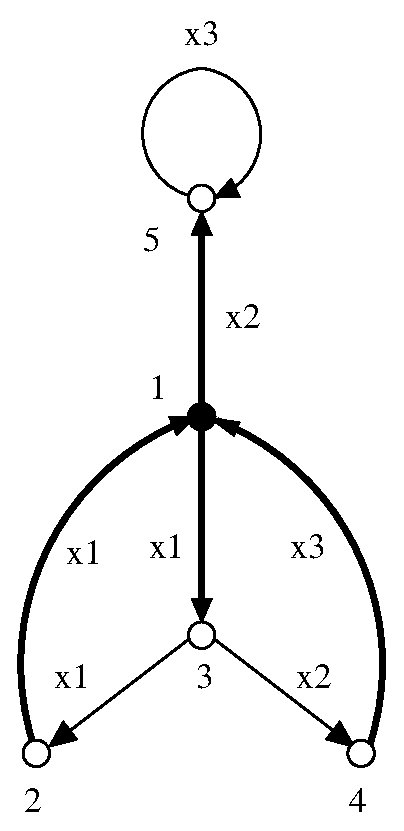
\includegraphics[scale=.52]{stallh1.eps}
\label{fig:stall1}} 
\hspace{5mm} 
\subfigure[$\G_{A_1}\times \G_{A_1}$: connected component of $(3,1)$.]{ 
\psfrag{a}{$(1,2)$}
\psfrag{b}{$(2,3)$}
\psfrag{c}{$(3,1)$}
\psfrag{d}{$(4,5)$}
\psfrag{e}{$(1,5)$}
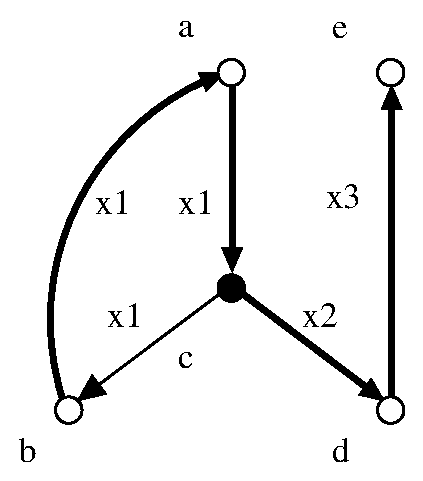
\includegraphics[scale=.52]{GxG-1.eps}
\label{fig:GxG-1}}
\hspace{5mm} 
\subfigure[$\G_{A_1}\times \G_{A_1}$: connected component of $(2,1)$.]{ 
\psfrag{a}{$(2,1)$}
\psfrag{b}{$(3,2)$}
\psfrag{c}{$(1,3)$}
\psfrag{d}{$(5,4)$}
\psfrag{e}{$(5,1)$}
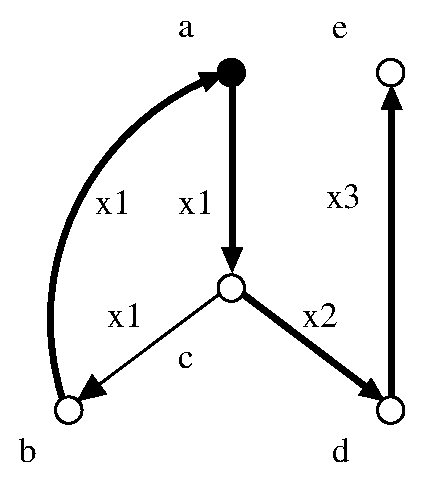
\includegraphics[scale=.52]{GxG-2.eps}
\label{fig:GxG-2}}
\end{center}
\caption{Example \ref{ex:f_1}.}\label{fig:stall}
\end{figure}

\begin{example}\label{ex:f_2}
Let $F_2$ be the free group on generators
$y_1,y_2,y_3,y_4$ with a subgroup $H_2 = \la h_1^{\prime},
h_2^{\prime},h_3^{\prime}\ra$, where 
$h_1^{\prime}=y_2^2$, 
$h_2^{\prime}=y_3y_4$ and  
$h_3^{\prime}=y_1^2y_3y_1^{-1}y_2$.
The Stallings automata, $\G_{A_2}$ for $H_2$,  
with maximal subtree $T_2$ highlighted and base vertex $1$, is shown
in Figure \ref{fig:stallagain}.\ref{fig:stallh2}. 
The set $L_{T_2}$ corresponding to the maximal subtree  $T_2$ is
 $L_{T_2}=
\{1, y_1, y_1^2,
y_2^{-1}, y_2^{-1}y_1, y_3 \}$.
Let the set of double coset representatives for $H_2$ be $S_2=S_2^{(1)}
\cup S_2^{(2)}$. 

To find the normal form of 
$f_3=y_1^2y_3y_1^{-1}y_2y_3y_4y_1y_2 y_3y_4y_2^2$: : use  
${A_2}$ to read off the maximal acceptable prefix 
$h= y_1^2y_3y_1^{-1}y_2y_3y_4$ of $f_3$; and  the maximal $L_{Q_2}$-prefix 
$p=y_1$ of the rest of $f_3$.  Next  
$q^{-1}= y_2^{-2}y_4^{-1}y_3^{-1}y_2^{-1}$, so $g=y_2^{-2}y_4^{-1}y_3^{-1}$
and $t=y_2^{-1}$. This element will be represented by an
element of $S_2^{(2)}$, so we need to construct $\G_{A_2}\times \G_{A_2}$. 
There are $7$  non-trivial, non-diagonal components. One is shown in Figure
\ref{fig:stallagain}\ref{fig:stallh2} and the remaining
six in  
Figure \ref{fig:G2xG2-2}. In all cases the solid vertex corresponds 
to the $\sim$ representative and connecting elements are paths in the
highlighted trees. Following Algorithm I, the normal form of $f_3$ is
seen to be 
\[f_3=h yz^{-1} g^{-1},\]
where $y=y_1$, $z=y_2$ and $yz^{-1}=y_1y_2^{-1}\in S_2^{(2)}$: that is 
\[f_3=h^\prime_3h_2^\prime y_1y_2^{-1} (h_1^\prime)^{-1}(h_2^\prime)^{-1}.\]
\end{example}

\begin{figure}
\begin{center}

\psfrag{y1}{$y_1$}

\psfrag{y2}{$y_2$}

\psfrag{y3}{$y_3$}

\psfrag{y4}{$y_4$}
\psfrag{1}{$1$}
\psfrag{2}{$2$}
\psfrag{3}{$3$}
\psfrag{4}{$4$}
\psfrag{5}{$5$}
\psfrag{6}{$6$}
\subfigure[Stallings automaton $A_2$ for $H_2$]{
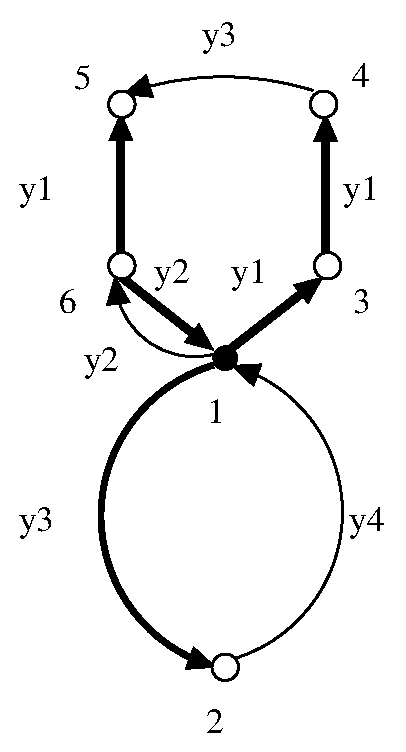
\includegraphics[scale=.52]{stallh2.eps}
\label{fig:stallh2}} 
\hspace{25mm} 
\subfigure[$\G_{A_2}\times \G_{A_2}$: connected component of
$(6,1)$.]{ 
\psfrag{a}{$(5,3)$}
\psfrag{b}{$(6,1)$}
\psfrag{c}{$(1,6)$}
\psfrag{d}{$(3,5)$}
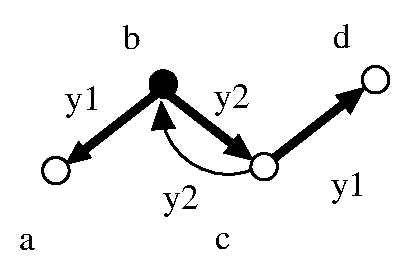
\includegraphics[scale=.52]{G2xG2-1.eps}
\label{fig:G2xG2-1}}
\end{center}
\caption{Stallings automata for Example \ref{ex:f_2}.}\label{fig:stallagain}
\end{figure}

\begin{figure}
\begin{center}

\psfrag{y1}{$y_1$}

\psfrag{y2}{$y_2$}

\psfrag{y3}{$y_3$}

\psfrag{y4}{$y_4$}
\psfrag{b}{$(1,3)$}
\psfrag{c}{$(3,4)$}
\subfigure[$(1,3)$.]{
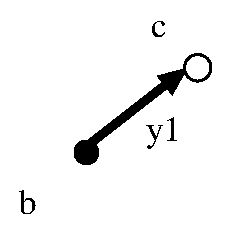
\includegraphics[scale=.5]{G2xG2-2.eps}
\label{fig:G2xG2-2-1}} 
\hspace{1mm} 
\subfigure[$(3,1)$.]{ 
\psfrag{b}{$(3,1)$}
\psfrag{c}{$(4,3)$}
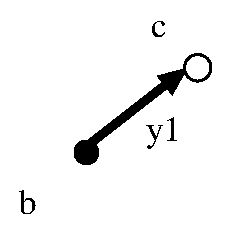
\includegraphics[scale=.5]{G2xG2-2.eps}
\label{fig:G2xG2-2-2}}
\hspace{1mm} 
\subfigure[$(2,5)$.]{
\psfrag{y1}{$y_3$}
\psfrag{b}{$(1,4)$}
\psfrag{c}{$(2,5)$}
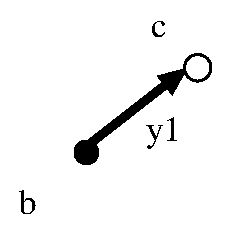
\includegraphics[scale=.5]{G2xG2-2.eps}
\label{fig:G2xG2-2-3}}
\hspace{1mm} 
\subfigure[$(5,2)$.]{ 
\psfrag{y1}{$y_3$}
\psfrag{b}{$(4,1)$}
\psfrag{c}{$(5,2)$}
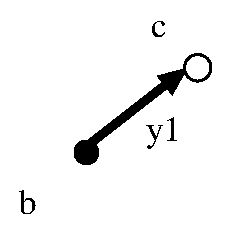
\includegraphics[scale=.5]{G2xG2-2.eps}
\label{fig:G2xG2-2-4}}
\hspace{1mm} 
\subfigure[$(4,5)$.]{
\psfrag{y1}{$y_1$} 
\psfrag{b}{$(3,6)$}
\psfrag{c}{$(4,5)$}
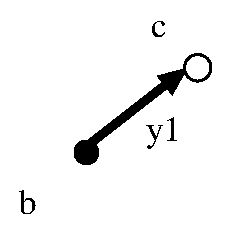
\includegraphics[scale=.5]{G2xG2-2.eps}
\label{fig:G2xG2-2-5}}
\hspace{1mm} 
\subfigure[$(6,3)$.]{ 
\psfrag{b}{$(6,3)$}
\psfrag{c}{$(5,4)$}
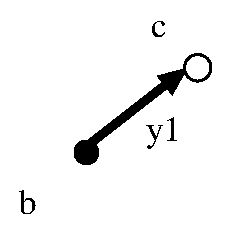
\includegraphics[scale=.5]{G2xG2-2.eps}
\label{fig:G2xG2-2-6}}
\end{center}
\caption{Example \ref{ex:f_2}: connected components of $\G_{A_2}\times \G_{A_2}$.}\label{fig:G2xG2-2}
\end{figure}

In fact if we don't require uniqueness of representatives then there is
a much simpler algorithm to write words in normal form.
This
simply finds the maximal prefix $h_1$ of $w$  accepted  by $A$  and so $w=h_1\circ v$. It then finds the
maximal prefix $p$ of $\bar v$ accepted by $A$. Setting $h_2=\bar p$ gives $w=h_1\circ d \circ h_2$, for
some uniquely determined word $d$, which is a (non-unique)
double coset representative.


%%
%%
%%As before let $g$ be a word in $F_1\ast F_2$ and suppose that
%%$g=g_1\cdots g_t$ in reduced form. Denote $S= S_1 \cup S_2$, where
%%$S_1$ are sets of double coset representatives for $H_1$ and $H_2$
%%correspondingly. Write each syllable $g_i$ of $g=g_1\cdots g_t$ in
%%normal form using the algorithm above. This gives
%%$g_i=h_{i,1}d_ih_{i,2}$, with $d_i\in S$ and $h_{i,j}\in H_1\cup
%%H_2$. Using $\phi_1^{-1}$ or $\phi_2^{-1}$, as appropriate, we now
%%write $h_{i,1}$ and $h_{i,2}$ as reduced words in $F(Z)$. For
%%$i=1,\ldots , t-1$, we reduce the word $h_{i,2}h_{(i+1),1}\in
%%F(Z)$ to give a reduced word $h_i\in F(Z)$ and set $h_0=h_{1,1}$
%%and  $h_{t+1}=h_{t,2}$. Then $g$ has normal form $h_0d_1h_1\cdots
%%d_th_{t+1}$.
%%
%%
%%\begin{example}\label{ex:g}
%%Let $g =f_1 f_2 f_1^{-1}$ in settings of Example \ref{ex:f_1f_2}.
%%Set $z_i = h_i = h_i^{\prime}$ for $i= 1,2,3$; then
%%
%%\begin{align*}
%%g &= (z_2^2z_1)\cdot x_1 \circ x_3^3x_1^{-1} \circ x_1^{-1}\cdot
%%(z_3^{-1}z_3^2z_2) \cdot y_1 \circ (y_2^{-1})^{-1}\\ &\cdot(z_2 z_1 z_3)\cdot x_1\circ x_1 x_3^{-3} \circ x_1^{-1}\cdot (z_1^{-1}z_2^{-2})=\\
%%&(z_2^2z_1)\cdot d_1(x) \cdot (z_3z_2) \cdot d_2(y) \cdot(z_2 z_1
%%z_3) \cdot d_1(x)^{-1} (z_1^{-1}z_2^{-2}).
%%\end{align*}
%%
%%
%%
%%\end{example}

%
%%%
%
%%%%%%%%%%%%%%%%%%%%%%%%%%%%%%%%%%%%%%%%%%%%%%%%%
\section{The generalised folding process}\label{sec:foldings}
The object is to construct an automaton which will accept a word
$w$ in double coset normal form if and only if it belongs to a
given subgroup $K$. The idea is to do this by starting with the
flower automaton for the generators of $K$, written in (double
coset) normal form; carrying out Stallings folding as usual to
produce a deterministic, trim, inversive automaton; and next
adding some additional paths to allow normal forms to be read.
This may introduce new non-determinism in some  states (i.e. edges
which may be folded), so the resulting automaton must be folded
again. The result of the final folding is the candidate automaton.

 Suppose $L$ is the
language accepted by the flower automaton of $K$. The image of $L$ under
the canonical map to $G$ is $K$. All the stages of our generalised folding
process will preserve this image, so our final automaton will accept a language
$L_1$ which also maps to $K$. We must then prove that if $w$ is a word
in normal form which represents an element of $K$ then $w$ is in $L_1$. It will
therefore suffice to show that if $u$ is any word in $L_1$ then the
normal form of $u$ is also in $L_1$.

Recall from above that we have $F_1$, $F_2$ free groups (finitely
generated by $X_1$ and $X_2$, respectively);
 $H_1 \leq F_1$, $H_2 \leq F_2$ such that
there exists an isomorphism $\phi: H_1 \rightarrow H_2$; a free group
 $F(Z)$, generated by $Z=\{z_1, \ldots, z_m\}$,
and  maps $\phi_1$ and $\phi_2$ such that $\phi_1(z_i)=h_i(X_1)  $
and  $\phi_2(z_i)=h^\prime_i(X_2)$, $i=1,\ldots ,m$, both of which
induce isomorphisms with $\phi=\phi_2\phi_1^{-1}$. Implicit in all
this is that $X_1\cap X_2=X_1\cap Z = X_2\cap Z=\nul$. We define
${G = F_1 \underset{H_1=H_2}{\ast} F_2}$, the group with
 presentation $\la X_1,X_2 | h_i = h_i', i=1 \ldots m\ra$ and
let $S_1$ and $S_2$ be sets of  double coset representatives of
$H_1\le F_1$ and $H_2\le F_2$, respectively, (as in Section
\ref{sec:intro}); denote $S= S_1 \cup S_2$. Let $A_k$ be the
Stallings automaton for $H_k$ and let $T_k$ be a spanning tree for
the associated graph $\G_{A_k}$, $k=1,2$. The alphabet of $A_k$ is
$X_k$ and the set of states of $A_k$ is denoted $Q_k$. 

%\subsection{Construction of the double coset normal form}\label{sub:construction_dcnf}}
Suppose that $g \in G$ and $g=g_1\cdots g_t$ is in reduced form.
Write each syllable $g_i$ of $g=g_1\cdots g_t$ in normal form
using the algorithm I above. This gives
$g_i=h_{i,1}d_ih_{i,2}$, with $d_i\in S$ and $h_{i,j}\in H_1\cup
H_2$. Using $\phi_1^{-1}$ or $\phi_2^{-1}$, as appropriate, we now
write $h_{i,1}$ and $h_{i,2}$ as reduced words in $F(Z)$. For
$i=1,\ldots , t-1$, we reduce the word $h_{i,2}h_{(i+1),1}\in
F(Z)$ to give a reduced word $h_i\in F(Z)$ and set $h_0=h_{1,1}$
and  $h_{t+1}=h_{t,2}$. Then $g$ has normal form $h_0d_1h_1\cdots
d_th_{t+1}$.


\begin{example}\label{ex:g}
Let $g =f_1 f_2 f_3 f_2^{-1}$ in setting  of Examples \ref{ex:f_1} and 
Examples \ref{ex:f_2}.
Set $z_i = h_i = h_i^{\prime}$ for $i= 1,2,3$; then
\begin{align*}
f_1&=(h_2^{2}h_1) x_1x_3x_1^{-1} (h_1^{-1}h_3^{-1})\\
&=z_2^2z_1  x_1x_3x_1^{-1}z_1^{-1}z_3^{-1},\\
f_2&=(h_3^{-1}h_2) x_1^{-1}\\
&=z_3^{-1}z_2 x_1^{-1}\textrm{ and }\\
f_3&=h^\prime_3h_2^\prime y_1y_2^{-1} (h_1^\prime)^{-1}(h_2^\prime)^{-1}\\
&= z_3z_2 y_1y_2^{-1} z_1^{-1}z_2^{-1}.
\end{align*}
Then 
\[g=z_2^2 z_1  x_1 x_3 x_1^{-1} z_1^{-1} z_3^{-2}
z_2 x_1^{-1} 
z_3z_2 y_1y_2^{-1} z_1^{-1}z_2^{-1}
x_1z_2^{-1}z_3.
\]
\end{example}



\subsection{Double coset automata}
%
%
Let $K=\la k_1, \ldots , k_s\ra$, where $k_i$ is an element of $G$
written in normal form: say
\begin{equation}\label{eq:k-form}
k_i= h_{i,0}t_{i,1}h_{i,1}\cdots t_{i,m_i}h_{i,m_i+1},
\end{equation}
with $h_{i,j}\in F(Z)$ and $t_{i,j}\in S_1\cup S_2$. Denote
by $\hat K$ the subgroup of  $F(X_1\cup X_2 \cup Z)$ generated by
$k_1, \ldots , k_s$. 
Let $\cF(K)$ be the flower automaton of $\hat K$, and let
$\G$ be the corresponding rooted graph. If $e$ is an edge of $\G$ then
$e$ is labelled by a letter (of $X_1\cup X_2 \cup Z$)
occuring in $h_{i,j}$ or $t_{i,j}$, for some $i,j$, as in
\eqref{eq:k-form}. If $e$ is labelled by a letter of $Z$ we say $e$ has {\em type} $Z$.
 %and define $c(e)=(0,0)$.
If $e$ is labelled by a letter of $X_k$ occuring in
$t_{i,j}$, we say $e$ has {\em type} $X_k$.

Now let $\G_K$ be the Stallings folding of the graph $\G$.  Then
 $\G_K$ is inverse and $\pi(L(\G_K))=K$. However
$L(\G_K)$ does not, in general, contain all normal forms of elements of $K$.
We wish to transform $\G_K$ to allow it to accept normal forms of 
elements of $K$. In outline this transformation process consists 
of repeating steps \ref{it:gf1} and \ref{it:gf2} below until all normal forms
are accepted. First, to facilitate the description of the
loop, let $\G_K=\G_K^{(0)}$ and let $n=0$. 
\be[Step 1.]
\item\label{it:gf1} Add new paths to $\G_K^{(n)}$ which allow normal forms of labels
of certain paths to be read. If at least one path has been added, 
call the result $\G_{K}^{(n+1)}$.  If no paths are added at this step,
halt and output  $\G_K^{(n)}$. 
\item\label{it:gf2} Fold  $\G_{K}^{(n+1)}$, add $1$ to $n$, and repeat Step \ref{it:gf1}.
\ee

Algorithm II below describes exactly how to carry out Step 1 of this loop.
Since Step 1 may run more than once,  the input to this algorithm is
assumed to be an
arbitrary inverse automaton $\D$, with alphabet $X_1\cup X_2\cup Z$ and  
$\pi(L(\D))=K$. We then show that, if we start as above
with $\G_K=\G_K^{(0)}$,  the loop halts, at some $n<\infty$;  
at which point $\G_K^{(n)}$ is an inverse automaton which accepts the
normal form of every element of $K$. \\[1em]

\noindent\textbf{Algorithm II}. \\

Let $\D$ be an inverse automaton, with alphabet $X_1\cup X_2\cup Z$ and 
start and final state $1$, such that
$\pi(L(\D))=K$.  
Let $\D_k$ be the graph formed from $\D$ by removing all edges of
type $X_{k^\prime}$, where $k\neq k^\prime$. An $X_k$ component of
$\D_k$ is the subgraph of $\D$ formed from a connected component
of $\D_k$ by removing all leaves which are incident to edges of
type $Z$, and then repeating the process till there are no such
leaves left. Given an $X_k$ component $\T$ of $\D_k$,  a
{\em boundary vertex} of $\T$ is defined to be a vertex
$\a$ such that $\a$ is incident, in $\D$, to a vertex which does not
belong to $\T$.  
 We shall modify each  $X_k$ component $\T$ of $\D_k$ so that if $p$ is a path,
from a  boundary vertex $u$  to a boundary vertex $v$ of $T$,   
then the normal form  of  the
label $l(p)$ of $p$ is the label of a path from $u$ to $v$. Throughout
the modification process we keep track of the boundary vertices, so that 
once modification is complete the $X_k$ components can be reassembled, by
attaching as they did in $\D$. The modification of $X_k$ components 
consists of five steps, producting new graphs $\T_1$, $\T_2$, $\T_3$, $\T_4$ and $\T_5$. 
In each case there is a canonical morphism $\theta_i$ from $\T_{i-1}$ to $\T_i$ and,
 (writing $\T=\T_0$)  
we define the {\em boundary vertices} of $\T_{i}$ to be the vertices $\theta_{i}(v)$
of $\T_i$, such that $v$ is a boundary vertex of $\T_{i-1}$. Moreover the
 images $\theta_i\circ \cdots\circ \theta_1(v)$ of vertices of $\T$ in $\T_i$ are 
called {\em vertices of} $\T$. \\[1em]

\noindent\textbf{Modification 1: $\T\leadsto \T_1$.}\\
 Let $\T$ be an $X_k$ component of $\D_k$. 
If $(\a,z,\b)$ is an edge of
$\T$ labelled by an element $z\in Z$ then add a path from $\a$ to
$\b$ labelled by $\phi_k(z)$ to the graph $\T$. Do this for all such edges, fold
the resulting graph 
and call the result $\T_1$. (See Figure \ref{fig:alg2-1}.) 
\begin{figure}
\begin{center}
\psfrag{a}{$\a$}
\psfrag{b}{$\b$}
\psfrag{h}{$z$}
\psfrag{w}{$w$}
\subfigure%[]
{
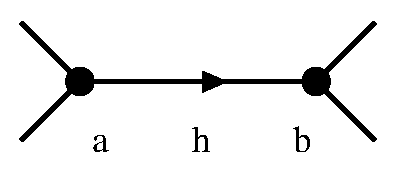
\includegraphics[scale=.5]{alg2-1a.eps}
\label{fig:alg2-1a}} 
\raisebox{3ex}{$\leadsto$}
\subfigure%[]
{ 
\psfrag{a}{$\a$}
\psfrag{b}{$\b$}
\psfrag{h}{$z$}
\psfrag{w}{$w$}
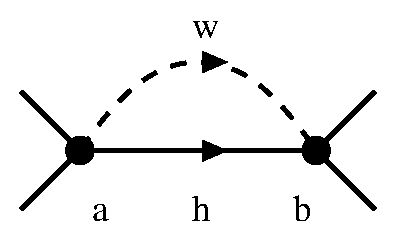
\includegraphics[scale=.5]{alg2-1b.eps}
\label{fig:alg2-1b}}
\end{center}
\caption{$\theta$ to $\theta_1$: $w=\phi_k(z)$}\label{fig:alg2-1}
\end{figure}
Let $\theta_1$ be the canonical
morphism from $\theta$ to $\theta_1$ and  define the boundary vertices of $\T_1$ to be
the vertices $\theta_1(v)$ of $T_1$, 
such that $v$ is a boundary vertex of $\T$. (We shall not mention this again in later
steps.)\\[1em]

\noindent\textbf{Modification 2: $\T_1\leadsto \T_2$.}\\
 Let $\cP_1=\T_1\times \G_{A_k}$. Then there is a path
 labelled $w$ from $\a$ to $\b$
in $\T_1$ and a path labelled $w$ from $\a^\prime $
to $\b^\prime$ in $\G_{A_k}$ if and only if there is a path
labelled $w$ from $(\a,\a^\prime)$ to $(\b,\b^\prime)$ in $\cP_1$.
 We shall
use this property of $\cP_1$ to determine which new paths to add  to
$\T_1$. Choose a spanning  forest $\U_1$ of  $\cP_1$. Next
 order the vertices of
$\T_1$: say these are $\a_0,\ldots, \a_t$, in the order written.

Let $\a_i$, $\a_j$ be vertices of  $\T$  with $i\le j$. If there
exists a simple path $p$ in $\cP_1$ from $(\a_i,1)$ to $(\a_j,1)$
then let $l_p\in F(X_k)$ be the label of $p$ and let
$w_p=\phi_k^{-1}(l_p)\in F(Z)$. Let $q$ be a path (disjoint from
$\T_1$) of length $|w_p|$ and with label $w_p$. Identify the
initial vertex of $q$ with $\a_i$ and the terminal vertex of $q$
with $\a_j$. (See Figure \ref{fig:alg2-2}.) 
\begin{figure}
\begin{center}
\psfrag{a}{$\a$}
\psfrag{b}{$\b$}
\psfrag{h}{$l_p$}
\psfrag{w}{$w_p$}
\psfrag{ai}{$(\a_i,1)$}
\psfrag{bi}{$(\a_j,1)$}
\psfrag{1}{$1$}
\psfrag{Th1 to Th2}{$\T_1\leadsto \T_2$}
\psfrag{cP}{$\cP_1$}
\psfrag{G_A}{$\G_{A_k}$}
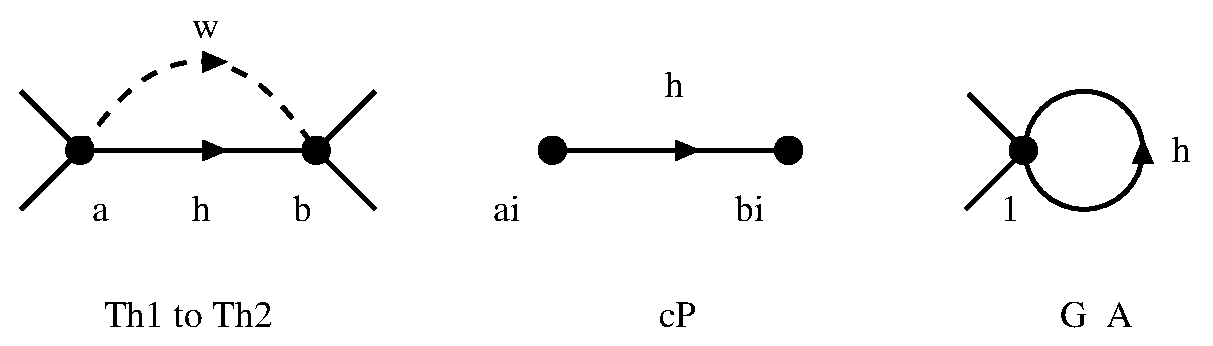
\includegraphics[scale=.5]{alg2-2.eps}
\end{center}
\caption{$\theta_1$ to $\theta_2$: $w_p=\phi_k^{-1}(l_p)$}\label{fig:alg2-2}
\end{figure}
Repeat this process for
all simple paths from  $(\a_i,1)$ to $(\a_j,1)$, over all pairs of
vertices $\a_i$, $\a_j$ of $\T$, with $i\le j$.  
There are finitely many simple paths in $\cP_1$ so this
process terminates. Call the result $\T_2^\prime$.
Then $\T_1$ is a subgraph of $T_2^\prime$. 
Now fold $\T_2^\prime$ to 
give a new graph 
$\T_2$. 
The composition $\theta_2$ 
of the the embedding map of $\T_1$ into $\T_2^\prime$ with the
canonical morphism from $\T_2^\prime$ to $\T_2$ is a morphism from $\T_1$ to
$\T_2$. 
 Moreover, if $\a$ and
 $\b$ are
boundary vertices of $\T_1$ and $L_1$ and $L_2$ are the
languages accepted by $(\T_1,\a,\b)$ and
$(\T_2,\theta_2(\a),\theta_2(\b))$, respectively, then 
by construction $\pi(L_1)=\pi(L_2)\subseteq G$.\\[1em]

\noindent\textbf{Modification 3: $\T_2\leadsto \T_3$.}\\
As the edges added to $\T_1$ to form $\T_2$ are all labelled by elements
of $Z$, and all edges of $\G_{A_k}$ are labelled by elements of $X_k$
the graphs $\cP_1=\T_1\times \G_{A_k}$ and $\cP_2=\T_2\times \G_{A_k}$ differ only
in that the second may have some new isolated vertices. Therefore we may
choose a spanning forest $\U_2$ of $\cP_2$ consisting of the spanning
forest $\U_1$ of $\cP_1$ with some new isolated vertices if necessary. 
If $\cP_2$ is a forest then 
$\cP_2=\U_2$, there is nothing to do at the
next stage, and we immediately set $\T_3=\T_2$. Otherwise, suppose
that $e$ is an edge of $\cP_2$ which does not belong to $\U_2$ but
which does belong to a component $\Xi$  of $\cP_2$ containing a
vertex $(\a,1)$, for some vertex $\a$ of $\T$. Let $(\a,1)$ be
such a vertex and let $e=((\a_i,\b_1), x, (\a_j,\b_2))$ be an edge
in same component of $\cP_2$ as $(\a,1)$,
 with label $x$ in $X_k$.
%Let
%$\a_m$ be the minimal vertex of $\T_2$ (necessarily also a vertex
%of $\T_1$)  such that $(\a_m,1)$ belongs to $\Xi$.
 Let $p_i$ be
the path in $\U_2$ from $(\a,1)$ to $(\a_i,\b_1)$ and let $p_j$ be
the path in $\U_2$ from  $(\a_j,\b_2)$ to $(\a,1)$ and
let $l_i$ and $l_j$ be the labels of $p_i$ and $p_j$, respectively. Then
$p_i,e,p_j$ projects to a closed path in $\G_{A_k}$, based at $1$, with
label $h_e=l_i x l_j \in H_k\subseteq F_k$. Moreover
$p_i,e,p_j$ projects to a closed path in $\T_2$, based at $\a$, also
with label $h_e$. Let
$w_e=\phi_k^{-1}(h_e)$ and let
$q$ be a path (disjoint from $\T_2$) of length
$|w_e|$ and with label $w_e$. Identify the initial and terminal
vertices of $q$ to the vertex  $\a$ of $\Theta_2$. Repeat this process for all such edges $e$ 
and
vertices $(\a,1)$ of $\cP_2$,  fold the
resulting graph, 
and denote the result by $\T_3$.
(In practice it's not necessary to
repeat this process for {\em all} such vertices $(\a,1)$ in $\Xi$: but it
makes some arguments  later easier if we assume that we do so.)
If
$L_3$ is the
language accepted by $(\T_3, \theta_3(\a),\theta_3(\b))$, for boundary
vertices $\a$, $\b$ of $\T_2$, then again $\pi(L_3)=\pi(L_2)$.


Next we wish to add paths to $\T_3$ that allow us to read the normal
forms of words $w$ which are readable by $\T_3$ and readable,
but not accepted, by $\G_{A_k}$.
As before we may assume that
$\cP=\T_1\times \G_{A_k}=
 \T_3\times \G_{A_k}$.
Recall that we have fixed a spanning subtree
$T_k$ of $\G_{A_k}$.
Let $\d=(\a_j,\b)$ be a vertex of $\cP$, with $\b\neq 1$, which lies
in a connected component of $\cP$ containing a vertex  $\g=(\a_i,1)$,
for some vertex $\a_i$ of $\T_3$.
Let $b$ be the label of the path in $T_k$ from $1$ to $\b$.
 If $\cP$ contains a simple
path from $(\a_i,1)$ to $(\a_j,\b)$, with label $b$,  then
 say that $\cP$ {\em covers} the pair $\g,\d$.
If all such pairs of vertices are covered by $\cP$ then set $\T_4=\T_3$.
Otherwise
let $p$ be the simple path in $\U$ from a
vertex $\g=(\a_i,1)$ to a vertex $\d=(\a_j,\b)$, where $\g,\d$
is not covered by $\cP$.
 Let
$p$ have label $a$.
Then $ab^{-1}=h\in H_k$. Let
$w=\phi_{k}^{-1}(ab^{-1})
\in F(Z)$ and let $q$ be a path (disjoint from $\T_3$)
with label $wb$. Identify the initial
and terminal vertices of $q$ with vertices $\a_i$ and $\a_j$ of $\T_3$,
respectively, and fold
the resulting graph.
As $\pi(a)=\pi(wb)\in G$ the image of the language accepted by
the resulting graph (considered as an automaton with start state  $\a_i$
 and final
state $\a_j$) is unchanged by
this operation.
Repeat this process for all pairs of  vertices which are not
covered by $\cP$ and
call the result $\T_4$.

Finally we wish to add paths which allow double coset representatives
of type $2$ to be read. Suppose $(\e,\xi)\in \G_{A_k}\times \G_{A_k}$ and
that the $\sim$ representative of $(\e,\xi)$ is $(\e_0,\xi_0)$.
Let $b_1$ and $b_2$ be the labels
of paths $w(\e)$ and $w(\xi)$, from $1$ to $\e$ and $1$ to $\xi$ in the
subtree $T_k$ of $\G_{A_k}$. Let $a_1$ and $a_2$ be the labels of
paths $w(\e_0)$ and $w(\xi_0)$. Then there are  paths in $\G_{A_k}$,
with label
$c=c(\e,\xi)$, from $\e$ to $\e_0$ and from $\xi$ to $\xi_0$.
Furthermore $h_i=
b_ica_i^{-1}\in H_k$ and $w_i=\phi_k^{-1}(h_i)\in F(Z)$, for $i=1,2$.
If there
exist paths $p_1$, with label $b_1$ from $(\a_i,1)$ to $(\a_j,\e)$,
and $p_2$, with label $b_2$ from
$(\a_l,1)$ to $(\a_j,\xi)$, in $\U$,  then
let $q$ be a path (disjoint from $\T_4$)
with label $w_1 a_1a_2^{-1} w_2^{-1}$,
and identify the initial
and terminal vertices of $q$ with  vertices $\a_i$ and $\a_l$
of $\T_4$, respectively.
Fold the resulting graph.
To see that the image of the language accepted by
 the new graph is the same as that of the original note
that the word $b_1b_2^{-1}$ is readable, starting at $\a_j$ and
ending at $\a_l$, in $\T_4$. As $\pi(b_1b_2^{-1})=\pi(w_1a_1a_2^{-1}w_2^{-1})$
the addition of this new path has no effect on the image, under $\pi$, of
the language accepted.
%$d_1$ and
%$d_2$ be labels of paths $p_1$ and $p_2$ in $\cP$ and let $e_1$ and
%$e_2$ be labels of simple paths with the same end points. Then
%$d_ie_i^{-1}\in H_k$ and  there is a path
%in $\T_4$ with label $\phi_k(d_ie_i^{-1})e_i$, for $i=1,2$. Moreover,
%$\T_4$ contains a path
%with label $\phi_k(e_ib_i^{-1})b_i$ and so a path with label
%$\phi(d_ib_i^{-1})b_i$, $i=1,2$.
Repeat this process for all such paths $p_i$ and $p_j$ and all such
pairs $(\e,\xi)$ to form $\T_5$.

\begin{lemma}
Let $\a$ and $\b$ be boundary vertices of $\T_1$ and let $w$ be a word
 which is accepted by the automaton $(\T_1, \a, \b)$. Then the
normal form of $w$ is accepted by $(\T_5, \a, \b)$.
\end{lemma}
\begin{proof}
We may assume that $w\in F(X_k)$ (given the construction of $\T_1$).
Let $w$ have normal form $h_1s h_2^{-1}$, where $s\in S_k$ and $h_i\in F(Z)$.
There are two cases to consider, depending on whether $s$ is a
representative of type $1$ or type $2$.
 First consider the case where $s$ is of type $1$, say
 $s= a_1 c a_2^{-1}$, where
$a_1$ is a maximal $L_{Q_k}$-prefix and an $L_{T_k}$ of $s$ and 
 $a_2$  is a maximal $L_{Q_k}$-prefix and an $L_{T_k}$ of $a_2\circ c^{-1}$. 
 Then there are words
$g_1, g_2, b_1$ and $b_2\in F(X_k)$ such that
$w=g_1\circ b_1\circ c \circ b_2^{-1}\circ g_2^{-1}$,
$g_i\in H_k$, $b_i$ is readable but not accepted by  $A_k$ and
$\phi_k(h_i)=g_ib_ia_i^{-1}$, $i=1,2$.

Since $g_i\in H_k$ and $w$ is accepted by $\T_1$ there is a path
labelled $g_1$ from $\a$ to a vertex $\a_1$ of $\T_1$ and a path
labelled $g_2$ from $\b$ to a vertex $\a_2$ of $\T_1$. Therefore, in $\cP$,
there are paths $p_1$ from $(\a,1)$ to $(\a_1,1)$ labelled $g_1$, and
$p_2$
from $(\b,1)$ to $(\a_2,1)$ labelled $g_2$.
Now $p_1$ may
be written as a concatenation of paths $p_1=o_0e_1\cdots e_l o_{l}$,
where $o_i$ is a simple path in $\U$ and $e_i$ is an edge of $\cP$ which does
not belong to $\U$.  Let $e_i$ have initial and terminal vertices
$\g_i$ and $\d_i$ and let $L_i$ and $R_i$ be the simple paths in $\U$ from
$(\a,1)$ to $\g_i$ and from $\d_i$ to $(\a,1)$, respectively.
Then, for $i=1,\ldots ,l$,
the path $L_i e_i R_i$ is a closed path in $\cP$, based
at $(\a,1)$, containing exactly one edge, $e_i$, which is not in $\U$.
Thus the label of  $L_i e_i R_i$ is $v_i\in H_k$ and $\phi_k^{-1}(v_i)$ is the
label of a closed path in $\T_3$, based at  $\a$. (All such paths
were added in the construction of $\T_3$ from $\T_2$.)
Also, there is a path $q_1$ in $\U$ from $(\a,1)$ to $(\a_1,1)$, with
label $v_{l+1}$, and by construction of $\T_2$ there is a path from $\a$ to
$\a_1$ in $\T_2$ with label $\phi_k^{-1}(v_{l+1})$.
The path
$p_1$ is the result of reducing (deleting adjacent edges $e,e^{-1}$) the path
$o_0 e_1 (R_1 R_1^{-1}) o_1 \cdots e_{l}(R_l R_l^{-1}) o_{l}$.
Moreover $o_0=L_1$; for $2\le i\le l$,
$L_i$ is the path obtained by reducing $R_{i-1}^{-1}o_{i-1}$; and
$R_{l}^{-1}o_{l}$ reduces to the path in $\U$ from
$(\a,1)$ to $(\a_1,1)$, that is to $q_1$.
Since the
order in which these reductions are carried out does not affect the end
result we may regard $p$ as the result of reducing the path
$L_1 e_1 R_1 \cdots L_l e_l R_l q_1$. Hence the label $g_1$
of $p_1$ is the result of
reducing the word $v_1\cdots v_l v_{l+1}$ and $\phi_k^{-1}(g_1)$ is the result of
reducing $\phi_k^{-1}(v_1) \cdots \phi_k^{-1}(v_{l+1})$. As each $\phi_k^{-1}(v_i)$ is readable
in $\T_3$ and $\T_3$ is folded this means  that $\phi_k^{-1}(g_1)$ is the
label of a path, from $\a$ to   $\a_1$, in $\T_3$. Similarly,
$\phi_k^{-1}(g_2)$
is the label of a path from $\b$ to $\a_2$ in $\T_3$.

The word $b_1$ is readable by $\G_{A_k}$ and there
is a path with label $b_1$ in $\T_1$ from $\a_1$ to some vertex $\b_1$.
Hence $b_1$ is the label of a path in $\cP$ from $(\a_1,1)$ to
$(\b_1,\e_1)$, for some vertex $\e_1$ of $\G_{A_k}$.
By definition $a_1$ is the label of a path in $T_k$ from $1$ to $\e_1$.
Let $b_1^\prime$
 be the label of the simple path $p_1^\prime$ in $\U$ from
$(\a_1,1)$ to $(\b_1,\e_1)$. By construction $\T_4$ contains a path
from $\a_1$ to $\b_1$ with label $h_1^\prime a_1$, where
$h_1^\prime =\phi_k^{-1}(b_1^\prime a_1^{-1})\in F(Z)$.
%(and is the empty word if $\cP$ covers $p^\prime$) and
%$b_1^{\prime\prime}$ is the label of the path in $T_k$ from $1$ to
%$\e_1$ (and equals $b_1^\prime$ if $\cP$ covers $p_1^\prime$).
(If $\cP$ covers the pair $(\a_1,1)$, $(\b_1,\e_1)$ then
$b_1^\prime=a_1$ and $h_1^\prime$ is the empty word.)
%Furthermore we have
%$\pi(\phi_k(h_1^\prime)b_1^{\prime\prime})=\pi(b_1^\prime)$.
Now $b_1(b_1^\prime)^{-1}\in H_k$ and is the label of a closed
path  in $\cP$ based at $(\a_1,1)$; so by the
previous part of proof, $\T_3$ contains a closed path, based at $\a_1$,
 with label
$w_1^\prime=\phi_k^{-1}(b_1(b_1^\prime)^{-1})$. Hence, as it is folded,
$\T_4$ contains a path, from $\a$ to $\b_1$,
with label the reduced word obtained from the product
$\phi_k^{-1}(g_1)w_1^{\prime} h_1^\prime a_1$, that is
 $\phi_k^{-1}(g_1b_1a_1^{-1}) a_1=h_1a_1$.
 Similarly, $\T_4$ contains a path from
$\b$ to $\b_2$ with label $h_2a_2$.

As $w$ is the label of a path in $\T_1$ there is a path from $\b_1$ to
$\b_2$ in $\T_4$ with label $c$. Therefore, in this case, $\T_4$ contains
a path from $\a$ to $\b$ which has label the normal form of $w$.

In the second case,
let $w$ have normal form $h_1 a_1 a_2^{-1} h_2^{-1} $, where
$h_1$ and $h_2$ are in $F(Z)$,  $a_1$ and $a_2$ are labels
of simple paths in the subtree $T_k$ and $a_1a_2^{-1}$ is a double coset
representative of type $2$. Then there are words
$g_1, g_2, k_1, k_2, b_1, b_2, c_1$ and $c_2\in F(X_k)$, uniquely
determined by $w$,  such that
$w=g_1\circ b_1 \circ b_2^{-1}\circ g_2^{-1}$,
$g_i, k_i\in H_k$, $b_i$ and $c_i$ are
readable but not accepted by  $A_k$, $c_i$ is the label of
a path in $T_k$, $b_ic_i^{-1}\in H_k$, $a_1a_2^{-1}=k_1c_1c_2^{-1}k_2^{-1}$
 and
$\phi_k(h_i)=g_ib_ic_i^{-1}k_i^{-1}$, $i=1,2$.
As in the first case the word $\phi_k^{-1}(g_1b_1c_1^{-1})c_1 c_2^{-1}
\phi_k^{-1}(c_2b_2^{-1}g_2^{-1})$ is readable in $\T_4$. By construction the
normal form $\phi_k^{-1}(k_1)a_1a_2^{-1}\phi_k^{-1}(k_2^{-1})$ of $c_1 c_2^{-1}$ is readable in
$\T_5$. It follows that the normal form of $w$ is readable in $\T_5$.
\end{proof}


Replace the subgraph $\T_1$ of $\D$ with $\T_5$, in the obvious
way. Carry through this procedure for each connected component of
$\D_k$, for $k=1$ and $2$. The resulting graph is said to be
obtained from $\D$ by {\em double coset resolution} or {\em dc-resolution}.


\begin{lemma}
Let $\D$ be  a connected, deterministic, trim, graph, let $\Phi$ be
the graph
obtained from $\D$ by dc-resolution %of attracting pairs
and let
$\L$ be the Stallings folding of $\Phi$. Then $\L$ is formed from
$\Phi$ by folding edges of type $Z$.
\end{lemma}
\begin{proof}
Let $\Phi=\L_0,\L_1,\ldots, \L_n$ be a sequence of graphs such that
$\L_{i+1}$ is obtained from $\L_i$ by and elementary folding.
Suppose that all these foldings except possibly the last involve only edges
of type $Z$. Assume $\L_n$ is formed from $\L_{n-1}$ by folding edges
$(\a,x,\b_1)$ and $(\a,x,\b_2)$ with label $x\in X_k$. Since the
first $n-1$ foldings involve only edges of type $Z$ it follows that
if $\g_1$ and $\g_2$ are vertices of $\Phi$ which map via these foldings
to $\b_1$ and $\b_2$, then there is a path $q$ in $\Phi$ from $\g_1$ to $\g_2$
which has label in $(Z^{\pm 1}\cup \{x^{\pm 1}\})^\ast$. Hence $\g_1$ and $\g_2$ both belong to
 the same $X_k$ component of $\Phi$, which also contains the path $q$.
Therefore all $n$ foldings can be carried out in this $X_k$
component. However the $X_k$ components of $\Phi$ are folded, since they
correspond to the graphs $\T_5$ constructed from $X_k$ components of $\D$.
Therefore no folding involving an edge of type $X_1$ or $X_2$ can occur
in such a sequence, and the result follows.
\end{proof}
\begin{lemma}
Let $\D$ be  a connected, deterministic, trim, graph, let $\Phi$ be
the graph
obtained from $\D$ by dc-resolution %of attracting pairs
and let
$\L$ be the Stallings folding of $\Phi$. Let $\a$  and $\b$ be boundary
vertices of an $X_k$ component of $\L$ and let $p$ be a path from
$\a$ to $\b$ with label $w\in F(X_k\cup Z)$. Then $\L$ contains a
path $q$ with label equal to the normal form of $w$.
\end{lemma}
\begin{proof}
Let $\g$ and $\d$ be vertices of $\Phi$ which map to $\a$ and $\b$ in the
folding of $\Phi$ to $\L$. As this folding involves only edges of type $Z$
it follows that $\g$ and $\d$ are in the same $X_k$ component of $\Phi$.
Moreover there is a path $p^\prime$ in $\Phi$ such that the image
of $p^\prime$ in $\L$ reduces to $p$. Then $\Phi$ contains a path
$q^\prime$ such that the label of $q^\prime$ is the normal form of
the label of $p^\prime$. Let $q$ be the reduced path in $\L$ obtained by
reduction of the image of $q^\prime$. Then the images of $l(q)$ and
$l(q^\prime)$ in $G$ are equal and both are equal to the image of $l(p)$ in
$G$. Moreover, since $l(q^\prime)$ is in normal form and $l(q)$ is obtained
from $l(q^\prime)$ by cancellation of letters of $Z$ it follows that
$l(q)$ is in normal form. Hence $l(q)$ is the normal form of $l(p)$,
as required.
\end{proof}
\begin{theorem}
Let $\cA=(\L,X_1\cup X_2\cup Z,\ast)$, where $\L$ is defined in the previous
lemma and $\ast$ is the root of $\L$. Then $\pi(L(\cA))=K$ and if $w$ is the normal form of an element
of $K$ then $w\in L(\cA)$.
\end{theorem}
\begin{proof}
We have $\pi(L(\cA))=\pi(L(\cF(K))=K$, by construction. If $u$ is a word
accepted by $\cA$ then we may write $u=z_0t_1z_1\cdots z_rt_rz_{r+1}$, where
$z_i\in F(Z)$ and $t_i$ is the label of a path between two boundary
vertices of an $X_1$ or $X_2$ component of $\L$, for all $i$. If
$s_i$ is the normal form of $t_i$ then, from the previous lemma, it follows
that $\cA$ also accepts the word $z_0s_1z_1\cdots z_rs_rz_{r+1}$, which
is the normal form of $u$.
\end{proof}
\begin{theorem}
$G$ has solvable subgroup membership problem.
\end{theorem}
%%%%%%%%%%%%%%%%%%%%%%%%%%%%%%%%%%%%%%%%%%%%%%%%%
\bibliographystyle{plain}
\bibliography{membership}

\medskip



\noindent \textsf{Andrew J. Duncan, School of Mathematics \&
Statistics, Newcastle University, Newcastle upon Tyne, NE1 7RU,
UK}

\noindent {\tt andrew.duncan@ncl.ac.uk}


\noindent \textsf{Elizaveta Frenkel, Moscow State University,
GSP-1, Leninskie gory, 119991, Moscow, Russia}

\noindent {\tt lizzy.frenkel@gmail.com}

\end{document}
